\documentclass{beamer}
\begin{document}
\begin{frame}
\begin{center}
    \Large\sc
     Every Tree Starts with a Root
\end{center}
    \begin{center}
    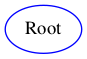
\includegraphics[width=2in]{G0.png}
    \end{center} 
\end{frame}

\begin{frame}
\begin{center}
    \Large\sc Trees Grow From A Root Following These Rules
\end{center}
\begin{enumerate}
\item The root gets left alone.
\item Every new dot you add gets connected to a dot that's already in the tree by an edge.
\item You always add dots in pairs, with each of the new dots connected to the same dot that's already in the tree.
\end{enumerate}
\begin{center}
    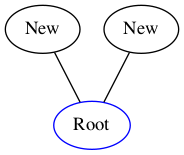
\includegraphics[width=2in]{G1.png}
    \end{center}
\end{frame}
\begin{frame}
   
    \begin{center}
        \Large Two trees with 5 dots and 4 lines
        
        \bigskip\noindent
    \begin{tabular}{cc}
    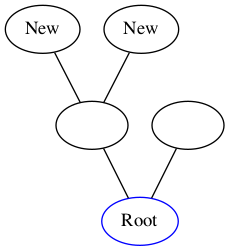
\includegraphics[width=2in]{G2.png} & 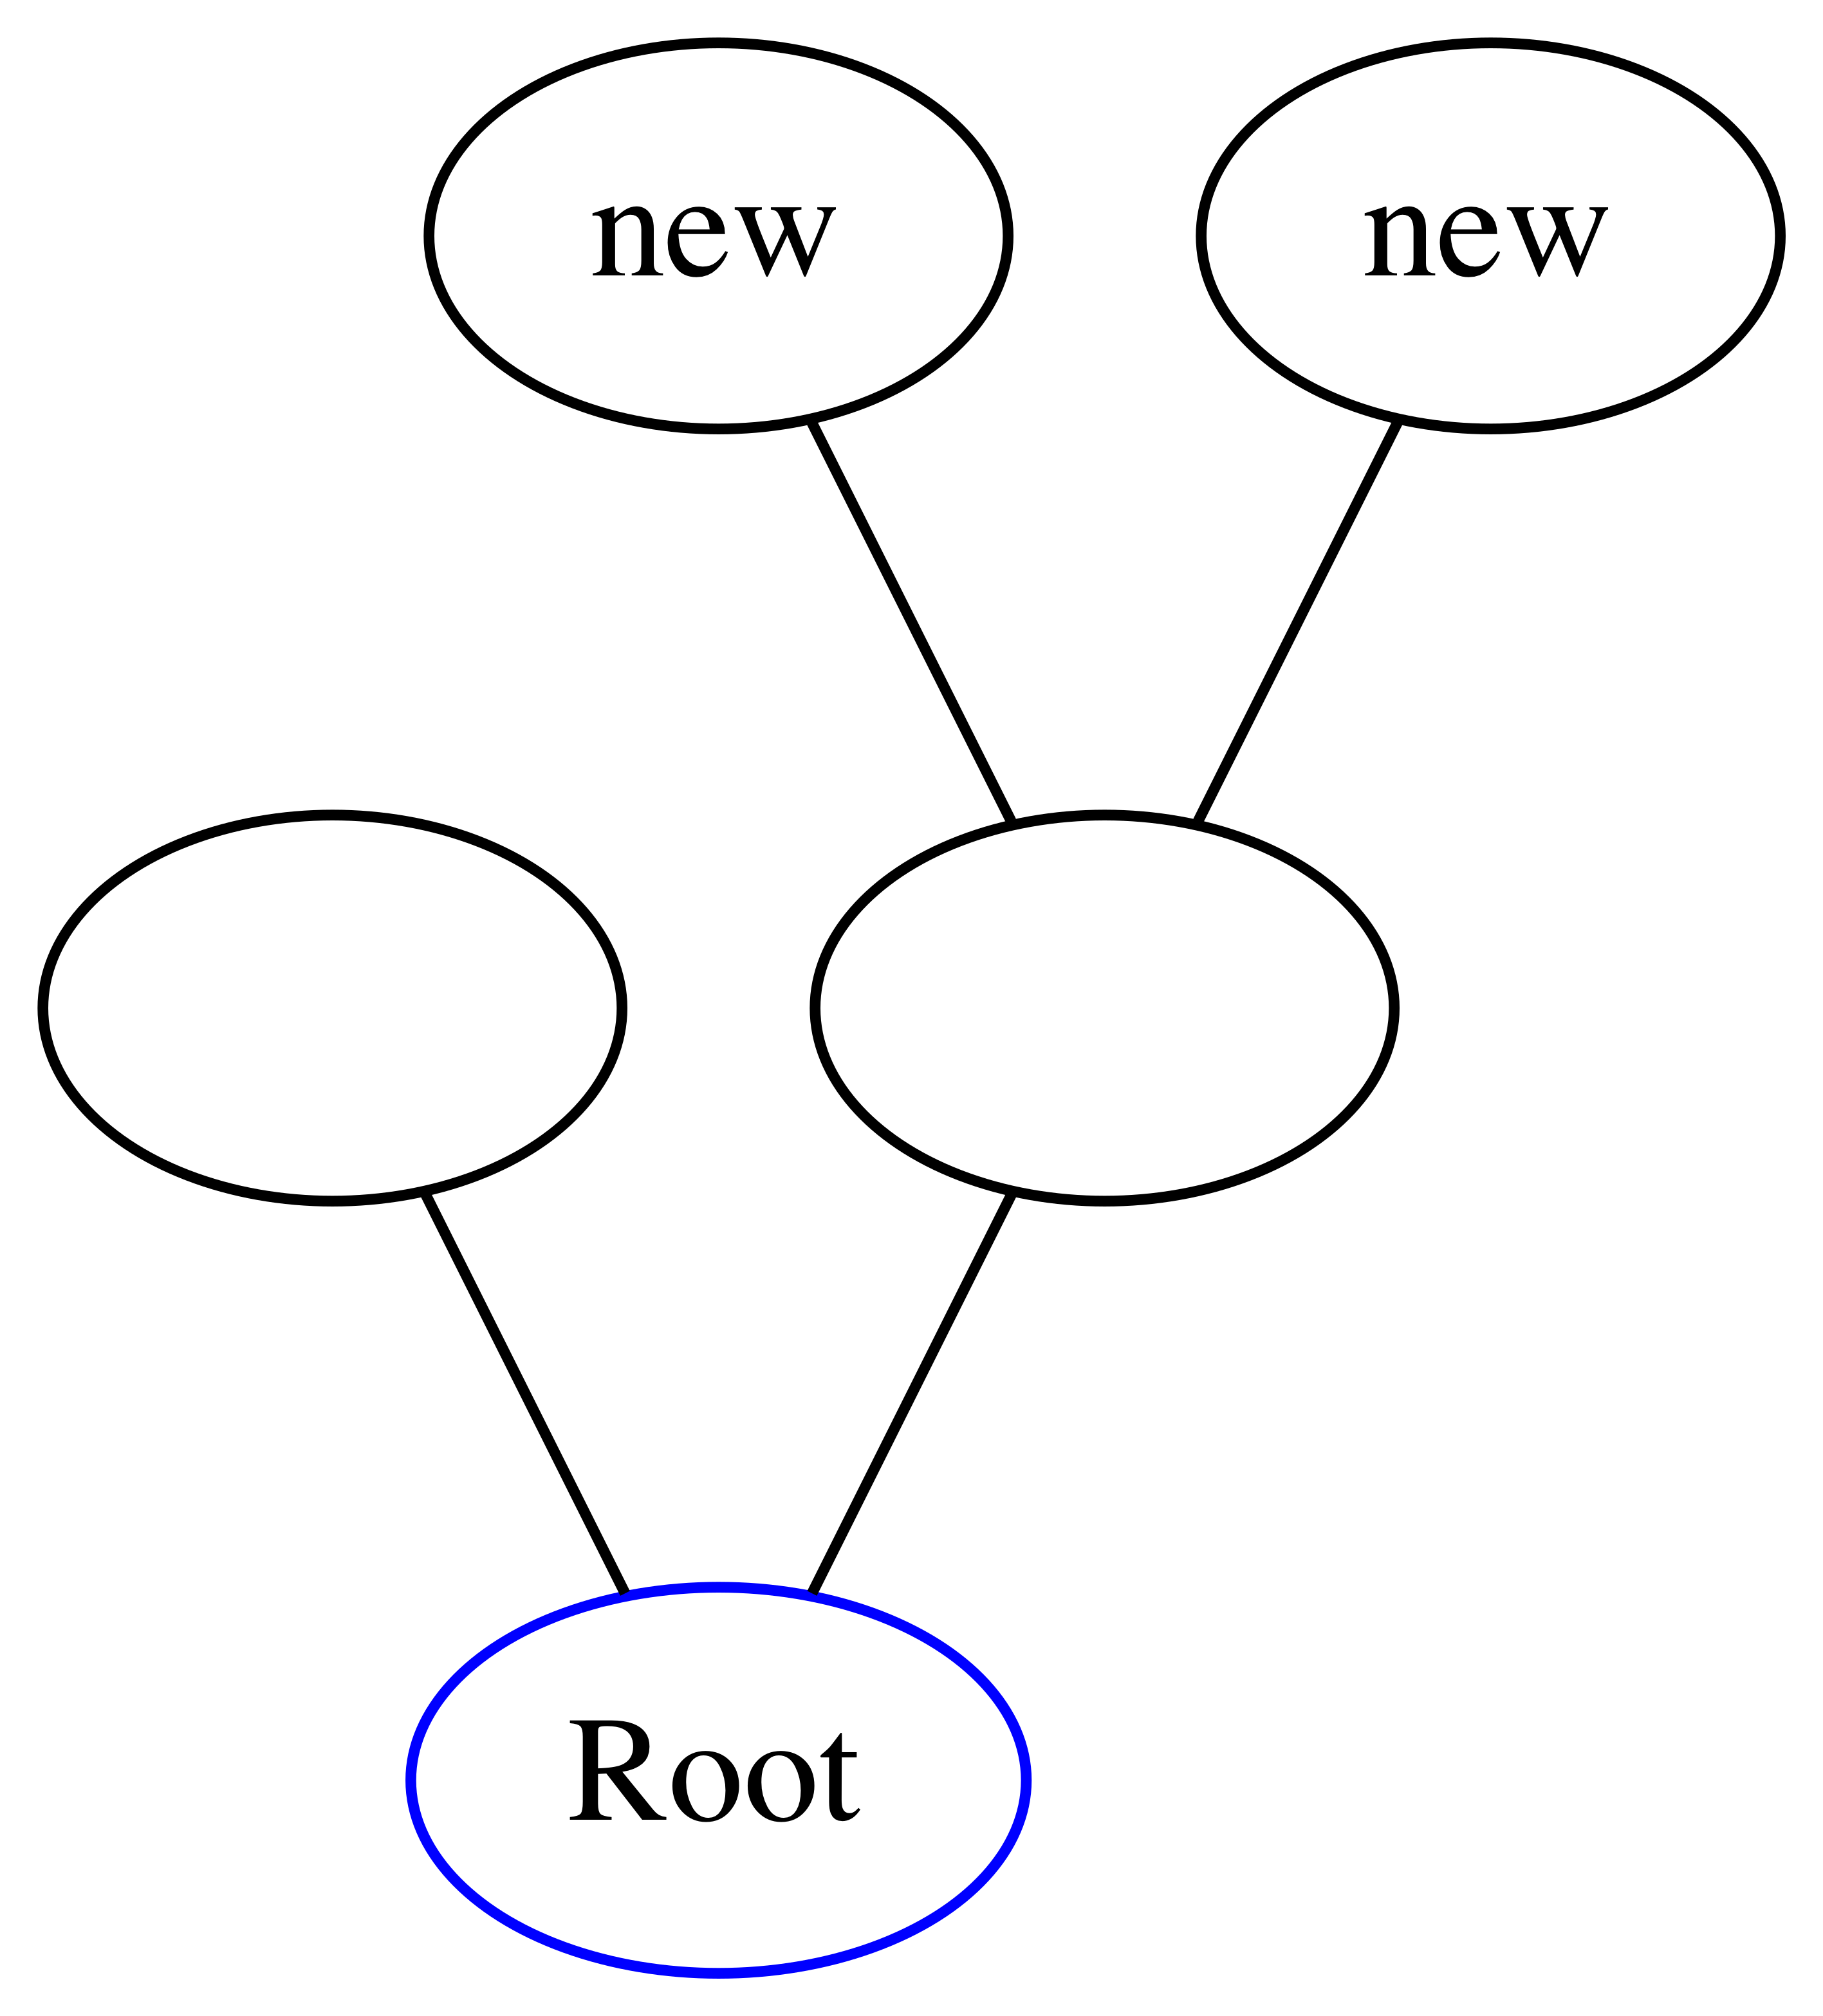
\includegraphics[width=2in]{G3.png}
    \end{tabular}
\end{center}
\end{frame}
\begin{frame}
\begin{center}
\Large Every Tree Always Satisfies These Rules
\end{center}
\begin{enumerate}
\item  A tree has a root dot at the bottom and either zero or two lines connected to it. 
\item Every dot in a tree except for the root has either three lines connected to it, or one.
\end{enumerate}
\begin{center}
\begin{tabular}{cc}
    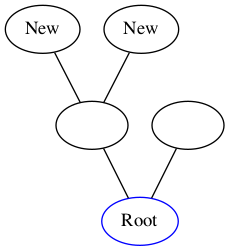
\includegraphics[height=1.5in]{G2.png} &  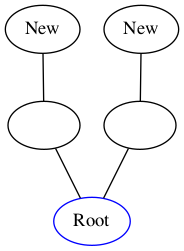
\includegraphics[height=1.5in]{G4.png} \\
    This is good! & This  breaks the rules!
\end{tabular}
 \end{center}
\end{frame}
\begin{frame}
    \begin{center}
    {\Large The BIG QUESTIONS}
    
    \bigskip\noindent
    {\Large How many \textit{DIFFERENT} trees are there with 3 dots?}
        (we'll talk about this)

    \bigskip\noindent
    {\Large How many \textit{DIFFERENT} trees are there with 5 dots?}
        (we'll talk about this)

    \bigskip\noindent
    {\Large How many \textit{DIFFERENT} trees are there with 7 dots?}
        (this is for you!)

    \bigskip\noindent
    {\Large How many \textit{DIFFERENT} trees are there with 9 dots?}
        (this is, too -- and it's tricky!)
    \end{center}

\end{frame}
\end{document}